% Options for packages loaded elsewhere
\PassOptionsToPackage{unicode}{hyperref}
\PassOptionsToPackage{hyphens}{url}
%
\documentclass[
]{article}
\usepackage{amsmath,amssymb}
\usepackage{iftex}
\ifPDFTeX
  \usepackage[T1]{fontenc}
  \usepackage[utf8]{inputenc}
  \usepackage{textcomp} % provide euro and other symbols
\else % if luatex or xetex
  \usepackage{unicode-math} % this also loads fontspec
  \defaultfontfeatures{Scale=MatchLowercase}
  \defaultfontfeatures[\rmfamily]{Ligatures=TeX,Scale=1}
\fi
\usepackage{lmodern}
\ifPDFTeX\else
  % xetex/luatex font selection
\fi
% Use upquote if available, for straight quotes in verbatim environments
\IfFileExists{upquote.sty}{\usepackage{upquote}}{}
\IfFileExists{microtype.sty}{% use microtype if available
  \usepackage[]{microtype}
  \UseMicrotypeSet[protrusion]{basicmath} % disable protrusion for tt fonts
}{}
\makeatletter
\@ifundefined{KOMAClassName}{% if non-KOMA class
  \IfFileExists{parskip.sty}{%
    \usepackage{parskip}
  }{% else
    \setlength{\parindent}{0pt}
    \setlength{\parskip}{6pt plus 2pt minus 1pt}}
}{% if KOMA class
  \KOMAoptions{parskip=half}}
\makeatother
\usepackage{xcolor}
\usepackage[margin=1in]{geometry}
\usepackage{color}
\usepackage{fancyvrb}
\newcommand{\VerbBar}{|}
\newcommand{\VERB}{\Verb[commandchars=\\\{\}]}
\DefineVerbatimEnvironment{Highlighting}{Verbatim}{commandchars=\\\{\}}
% Add ',fontsize=\small' for more characters per line
\usepackage{framed}
\definecolor{shadecolor}{RGB}{248,248,248}
\newenvironment{Shaded}{\begin{snugshade}}{\end{snugshade}}
\newcommand{\AlertTok}[1]{\textcolor[rgb]{0.94,0.16,0.16}{#1}}
\newcommand{\AnnotationTok}[1]{\textcolor[rgb]{0.56,0.35,0.01}{\textbf{\textit{#1}}}}
\newcommand{\AttributeTok}[1]{\textcolor[rgb]{0.13,0.29,0.53}{#1}}
\newcommand{\BaseNTok}[1]{\textcolor[rgb]{0.00,0.00,0.81}{#1}}
\newcommand{\BuiltInTok}[1]{#1}
\newcommand{\CharTok}[1]{\textcolor[rgb]{0.31,0.60,0.02}{#1}}
\newcommand{\CommentTok}[1]{\textcolor[rgb]{0.56,0.35,0.01}{\textit{#1}}}
\newcommand{\CommentVarTok}[1]{\textcolor[rgb]{0.56,0.35,0.01}{\textbf{\textit{#1}}}}
\newcommand{\ConstantTok}[1]{\textcolor[rgb]{0.56,0.35,0.01}{#1}}
\newcommand{\ControlFlowTok}[1]{\textcolor[rgb]{0.13,0.29,0.53}{\textbf{#1}}}
\newcommand{\DataTypeTok}[1]{\textcolor[rgb]{0.13,0.29,0.53}{#1}}
\newcommand{\DecValTok}[1]{\textcolor[rgb]{0.00,0.00,0.81}{#1}}
\newcommand{\DocumentationTok}[1]{\textcolor[rgb]{0.56,0.35,0.01}{\textbf{\textit{#1}}}}
\newcommand{\ErrorTok}[1]{\textcolor[rgb]{0.64,0.00,0.00}{\textbf{#1}}}
\newcommand{\ExtensionTok}[1]{#1}
\newcommand{\FloatTok}[1]{\textcolor[rgb]{0.00,0.00,0.81}{#1}}
\newcommand{\FunctionTok}[1]{\textcolor[rgb]{0.13,0.29,0.53}{\textbf{#1}}}
\newcommand{\ImportTok}[1]{#1}
\newcommand{\InformationTok}[1]{\textcolor[rgb]{0.56,0.35,0.01}{\textbf{\textit{#1}}}}
\newcommand{\KeywordTok}[1]{\textcolor[rgb]{0.13,0.29,0.53}{\textbf{#1}}}
\newcommand{\NormalTok}[1]{#1}
\newcommand{\OperatorTok}[1]{\textcolor[rgb]{0.81,0.36,0.00}{\textbf{#1}}}
\newcommand{\OtherTok}[1]{\textcolor[rgb]{0.56,0.35,0.01}{#1}}
\newcommand{\PreprocessorTok}[1]{\textcolor[rgb]{0.56,0.35,0.01}{\textit{#1}}}
\newcommand{\RegionMarkerTok}[1]{#1}
\newcommand{\SpecialCharTok}[1]{\textcolor[rgb]{0.81,0.36,0.00}{\textbf{#1}}}
\newcommand{\SpecialStringTok}[1]{\textcolor[rgb]{0.31,0.60,0.02}{#1}}
\newcommand{\StringTok}[1]{\textcolor[rgb]{0.31,0.60,0.02}{#1}}
\newcommand{\VariableTok}[1]{\textcolor[rgb]{0.00,0.00,0.00}{#1}}
\newcommand{\VerbatimStringTok}[1]{\textcolor[rgb]{0.31,0.60,0.02}{#1}}
\newcommand{\WarningTok}[1]{\textcolor[rgb]{0.56,0.35,0.01}{\textbf{\textit{#1}}}}
\usepackage{graphicx}
\makeatletter
\def\maxwidth{\ifdim\Gin@nat@width>\linewidth\linewidth\else\Gin@nat@width\fi}
\def\maxheight{\ifdim\Gin@nat@height>\textheight\textheight\else\Gin@nat@height\fi}
\makeatother
% Scale images if necessary, so that they will not overflow the page
% margins by default, and it is still possible to overwrite the defaults
% using explicit options in \includegraphics[width, height, ...]{}
\setkeys{Gin}{width=\maxwidth,height=\maxheight,keepaspectratio}
% Set default figure placement to htbp
\makeatletter
\def\fps@figure{htbp}
\makeatother
\setlength{\emergencystretch}{3em} % prevent overfull lines
\providecommand{\tightlist}{%
  \setlength{\itemsep}{0pt}\setlength{\parskip}{0pt}}
\setcounter{secnumdepth}{-\maxdimen} % remove section numbering
\usepackage{booktabs}
\usepackage{longtable}
\usepackage{array}
\usepackage{multirow}
\usepackage{wrapfig}
\usepackage{float}
\usepackage{colortbl}
\usepackage{pdflscape}
\usepackage{tabu}
\usepackage{threeparttable}
\usepackage{threeparttablex}
\usepackage[normalem]{ulem}
\usepackage{makecell}
\usepackage{xcolor}
\usepackage{siunitx}

  \newcolumntype{d}{S[
    input-open-uncertainty=,
    input-close-uncertainty=,
    parse-numbers = false,
    table-align-text-pre=false,
    table-align-text-post=false
  ]}
  
\ifLuaTeX
  \usepackage{selnolig}  % disable illegal ligatures
\fi
\IfFileExists{bookmark.sty}{\usepackage{bookmark}}{\usepackage{hyperref}}
\IfFileExists{xurl.sty}{\usepackage{xurl}}{} % add URL line breaks if available
\urlstyle{same}
\hypersetup{
  pdftitle={Marginal effects: a horrible mess and how to use it},
  pdfauthor={Doug Sponsler},
  hidelinks,
  pdfcreator={LaTeX via pandoc}}

\title{Marginal effects: a horrible mess and how to use it}
\author{Doug Sponsler}
\date{2023-10-27}

\begin{document}
\maketitle

\hypertarget{a-conversation}{%
\section{A conversation}\label{a-conversation}}

Dear Andrew,

First of all, thank you so much for all the work you put into your blog.
It's the best resource I have found for the sort of modeling questions I
encounter in my work.

If I may, I have a question concerning the definitions of ``marginal''
vs.~``conditional'' effects. I have encountered what would appear to be
at least three alternative definitions:

\begin{enumerate}
\def\labelenumi{\arabic{enumi}.}
\item
  In your post
  \href{https://www.andrewheiss.com/blog/2022/05/20/marginalia/}{``Marginalia''},
  you use the ``slider'' vs.~``switch'' analogy; marginal effects are
  partial derivatives for continuous variables, while conditional
  effects are discrete ``deltas'' associated with factor levels. Fair
  enough --- a good, clean definition.
\item
  In your more recent
  \href{https://www.andrewheiss.com/blog/2022/11/29/conditional-marginal-marginaleffects/}{post},
  you discuss how the terms marginal and conditional take on a different
  meaning in the context of hierarchical modeling. If I understand
  correctly, conditional effects are based solely on the fixed terms of
  the model, while marginal effects (somehow) incorporate the
  uncertainty arising from the random effects.
\item
  In the documentation of \texttt{ggeffects}, Daniel Lüdecke offers what
  would seem to be yet another definition: ``{[}The{]} effects returned
  by ggpredict() can be described as conditional effects (i.e.~these are
  conditioned on certain levels of factors), while ggemmeans() and
  ggeffect() return marginal means, since the effects
  are''marginalized'' (or ``averaged'') over the levels of factors.''
\end{enumerate}

I'd be very grateful for any light you can shed on this.

Best,

Doug

\begin{center}\rule{0.5\linewidth}{0.5pt}\end{center}

Hello!

Unfortunately all three definitions are true 😭

So marginal effects can refer to little changes in a slider (partial
derivatives, or differential calculus), and also to ``marginalizing''
and averaging across variables and finding marginal means, like the
\{ggeffects\} definition (averages, or integral calculus). The same word
means opposite concepts(!). PLUS in the multilevel model paradigm, it
refers to dealing with (or not dealing with) random effects.

It's all a horrible mess.

Andrew Heiss

\hypertarget{the-abyss-stares-back}{%
\section{The abyss stares back}\label{the-abyss-stares-back}}

Marginal and conditional effects are about what we \emph{do} with models
once we've gone through all the trouble of making them. All this
depends, of course, on understanding how your model works in the first
place, and how it relates to the world that it supposedly represents.

For us ecologists, working through all this is a healthy exercise. Our
workflow typically goes something like this. You begin with an
understanding of the world that inspires you to measure things. Having
gotten your measurements, you place your understanding of the world
safely on a shelf somewhere and proceed to the ``real work'' of doing
stats with your measurements. Pretty soon you realize that those t-tests
you learned in stats class aren't going to help. Your adviser shows you
how to use \texttt{aov()} to produce tables that you don't understand.
Then somebody introduces you to the \texttt{lm()} function and says that
\texttt{aov()} is totally passé, something about effect sizes, the
1990s, Nirvana, etc. You nod politely and get to work. Just when you
finish saving \texttt{analysis\_final\_final\_v2.r}, somebody asks you
why you're fitting a Gaussian model to count data. The real question,
you think to yourself, is why I'm doing this PhD program\ldots but you
smile and nod and try \texttt{glm()} instead. Now your model is spitting
out \emph{completely} different numbers, but some of the p-values still
look alright, so you breathe a sigh of relief and start writing your
results section. Then your adviser, who has just now looked at that
preliminary report you sent 3 months ago, asks why you didn't include
region as a covariate in your model, because that's how he did it in
that \emph{Ecology} paper from 1995. This triggers painful flashbacks
about \texttt{aov()} and the Backstreet Boys, but you recover and ask
Google what to do with categorical variables. A jolly looking bearded
chap named Ben Bolker keeps writing about ``mixed effects models'' and
some package called \texttt{lme4}, so, with a \texttt{glmer()} of hope,
you turn to \texttt{analysis\_final\_final\_v13.rmd} (because somebody
told you should try RMarkdown) and figure where the \textbar{} symbol is
on your keyboard. You press ctrl-enter, and your world falls apart.
Whatever ``convergence'' means, it's not happening. The summary table
gives you the impression that \texttt{aov()} is taking revenge for all
the bad things you've said about it. Worst of all, the p-values are just
\emph{gone}, vanished without a trace. You begin hallucinating. Four
months later, sunshine and birdsong wake you from your stats coma.
Spring has come again. Gandalf and Sam are standing by your bedside. To
your surprise, you look at
\texttt{analysis\_final\_final\_v37\_fuckfuck\_vfsebhvfehkbfsdjkhbjnlmk.qt}
(Quarto evidently came along during your coma) and discover what looks
like a working model. It has p-values. It has diagnostic plots that
aren't so bad. In your delirium, you made beautiful plots with
gracefully sweeping curves and stout, self-assured boxplots. Gingerly,
you take your understanding of the world from its shelf, blow off a
layer of dust, and begin to write\ldots{}

Okay, maybe that's a bit of an exaggeration. Maybe your experience
hasn't been as traumatic as mine. But the point is that understanding
marginal and conditional effects will require a deep dive into things
you may have never fully understood about your models. Hang on tight.

\hypertarget{a-disclaimer}{%
\section{A disclaimer}\label{a-disclaimer}}

Please note that throughout this demonstration, I will be ignoring
completely the issue of causal inference, which is the most important
thing about any statistical analysis (at least in ecology). The point is
just to illustrate the behavior of models.

\hypertarget{packages}{%
\section{Packages}\label{packages}}

\begin{Shaded}
\begin{Highlighting}[]
\CommentTok{\# Data}
\FunctionTok{library}\NormalTok{(palmerpenguins)}

\CommentTok{\# Frequentist modeling and visualization}
\FunctionTok{library}\NormalTok{(lme4)}
\FunctionTok{library}\NormalTok{(mgcv)}
\FunctionTok{library}\NormalTok{(ggeffects)}

\CommentTok{\# Bayesian modeling and visualization}
\FunctionTok{library}\NormalTok{(brms)}
\FunctionTok{library}\NormalTok{(tidybayes)}
\FunctionTok{library}\NormalTok{(ggdist)}

\CommentTok{\# Post{-}hoc analyses}
\FunctionTok{library}\NormalTok{(emmeans)}
\FunctionTok{library}\NormalTok{(marginaleffects)}

\CommentTok{\# Handling and visualization}
\FunctionTok{library}\NormalTok{(tidyverse)}
\FunctionTok{library}\NormalTok{(ggthemes)}
\FunctionTok{library}\NormalTok{(tidymodels)}
\FunctionTok{library}\NormalTok{(modelsummary)}
\FunctionTok{library}\NormalTok{(modelr)}
\FunctionTok{library}\NormalTok{(see)}
\end{Highlighting}
\end{Shaded}

\hypertarget{an-introduction-to-the-data}{%
\section{An introduction to the
data}\label{an-introduction-to-the-data}}

You might be wondering what the \texttt{palmerpenguins} dataset is
about. If you guessed penguins, you're right. After reading the data in
from the \texttt{palmerpenguins} package, we have a data frame called
\texttt{penguins}. We need to make one quick modification. In the
original data, the variable \texttt{year*} is coded as an integer
column. We want to change \texttt{year} to a factor column so that we
can treat it as a discrete rather than continuous variable, and we can
do this in one line with a call to \texttt{dplyr::mutate}.

\begin{Shaded}
\begin{Highlighting}[]
\FunctionTok{data}\NormalTok{(}\StringTok{"penguins"}\NormalTok{, }\AttributeTok{package =} \StringTok{"palmerpenguins"}\NormalTok{) }\CommentTok{\# read in data from package }

\NormalTok{penguins }\OtherTok{\textless{}{-}}\NormalTok{ penguins }\SpecialCharTok{\%\textgreater{}\%}
  \FunctionTok{mutate}\NormalTok{(}\AttributeTok{year =} \FunctionTok{factor}\NormalTok{(year)) }\CommentTok{\# convert \textasciigrave{}year\textasciigrave{} to factor}
\end{Highlighting}
\end{Shaded}

\begin{figure}
\centering
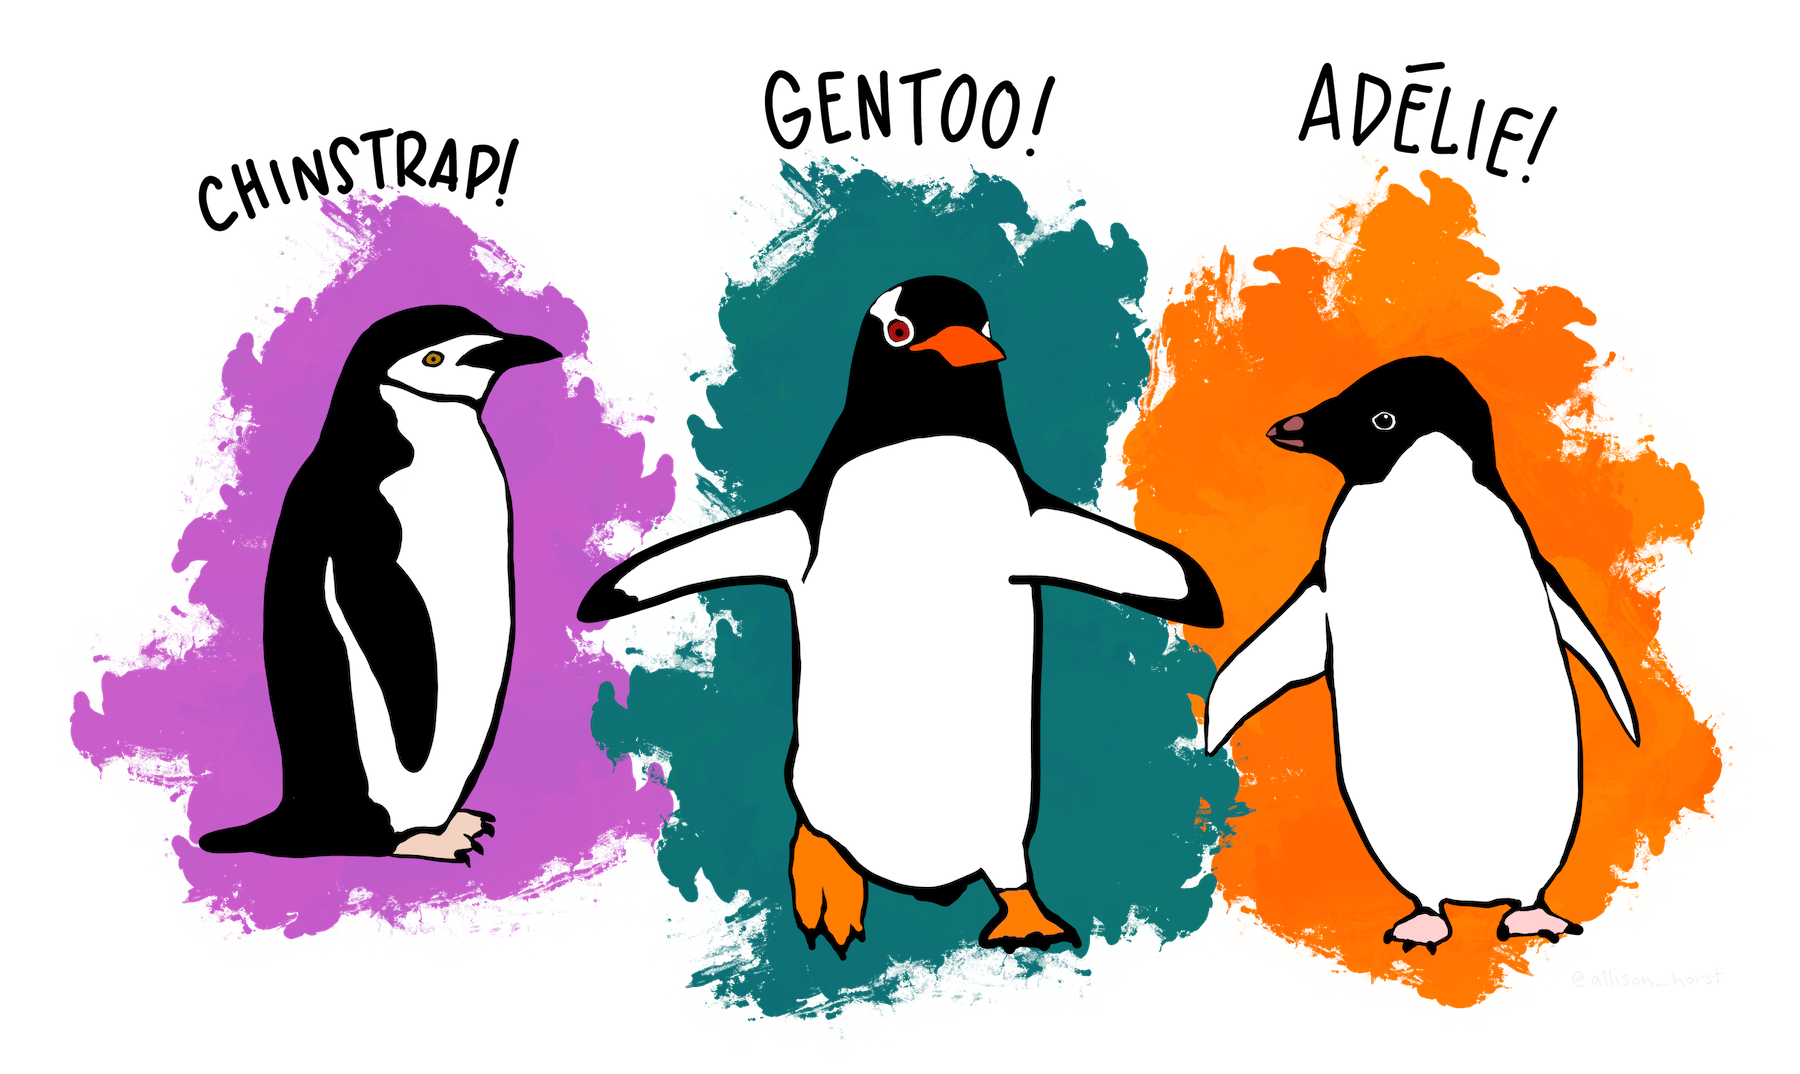
\includegraphics{./penguins.png}
\caption{Artwork by @allison\_horst}
\end{figure}

\begin{Shaded}
\begin{Highlighting}[]
\FunctionTok{datasummary\_skim}\NormalTok{(penguins, }\AttributeTok{type =} \StringTok{"categorical"}\NormalTok{)}
\end{Highlighting}
\end{Shaded}

\begin{table}
\centering
\begin{tabular}[t]{llrr}
\toprule
  &    & N & \%\\
\midrule
species & Adelie & 152 & \num{44.2}\\
 & Chinstrap & 68 & \num{19.8}\\
 & Gentoo & 124 & \num{36.0}\\
island & Biscoe & 168 & \num{48.8}\\
 & Dream & 124 & \num{36.0}\\
 & Torgersen & 52 & \num{15.1}\\
sex & female & 165 & \num{48.0}\\
 & male & 168 & \num{48.8}\\
year & 2007 & 110 & \num{32.0}\\
 & 2008 & 114 & \num{33.1}\\
 & 2009 & 120 & \num{34.9}\\
\bottomrule
\end{tabular}
\end{table}

\begin{figure}
\centering
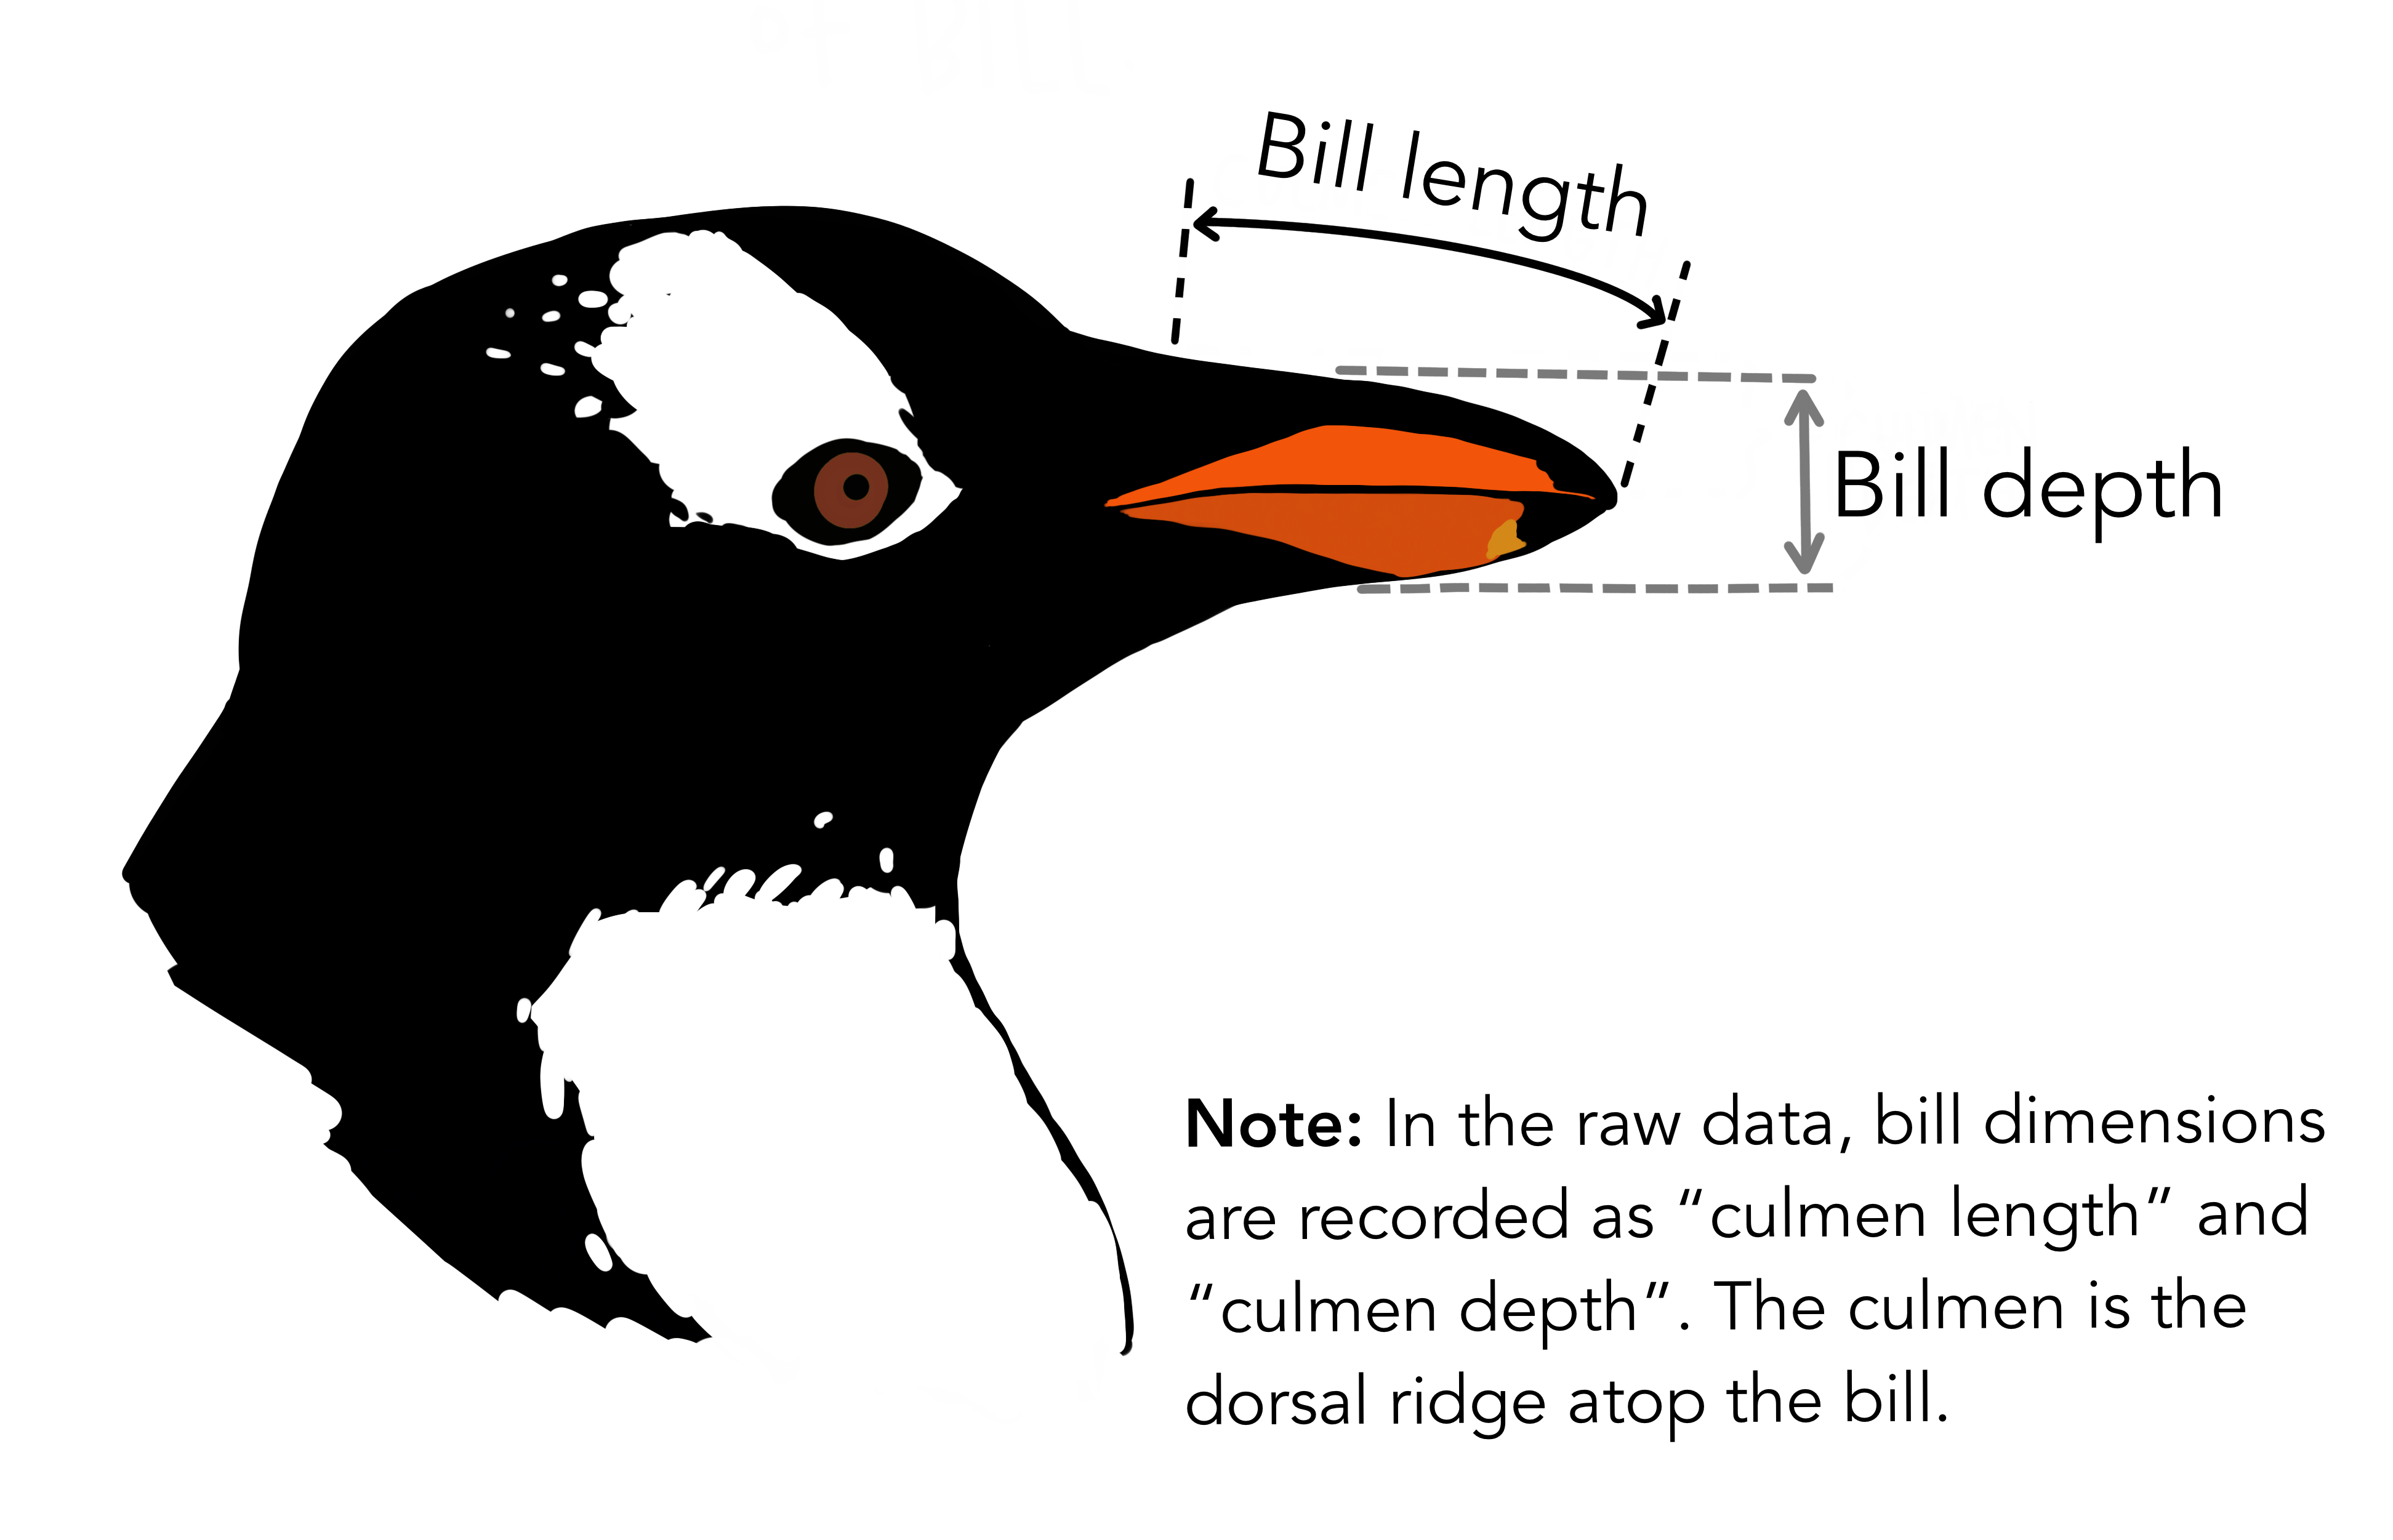
\includegraphics{./culmen_depth.png}
\caption{Artwork by @allison\_horst}
\end{figure}

\begin{Shaded}
\begin{Highlighting}[]
\FunctionTok{datasummary\_skim}\NormalTok{(penguins, }\AttributeTok{type =} \StringTok{"numeric"}\NormalTok{)}
\end{Highlighting}
\end{Shaded}

\begin{table}
\centering
\begin{tabular}[t]{lrrrrrrr>{}r}
\toprule
  & Unique (\#) & Missing (\%) & Mean & SD & Min & Median & Max &   \\
\midrule
bill\_length\_mm & 165 & 1 & \num{43.9} & \num{5.5} & \num{32.1} & \num{44.5} & \num{59.6} & \includegraphics[width=0.67in, height=0.17in]{demo_files/figure-latex//hist_47ea6812514b.pdf}\\
bill\_depth\_mm & 81 & 1 & \num{17.2} & \num{2.0} & \num{13.1} & \num{17.3} & \num{21.5} & \includegraphics[width=0.67in, height=0.17in]{demo_files/figure-latex//hist_47ea3d4db36.pdf}\\
flipper\_length\_mm & 56 & 1 & \num{200.9} & \num{14.1} & \num{172.0} & \num{197.0} & \num{231.0} & \includegraphics[width=0.67in, height=0.17in]{demo_files/figure-latex//hist_47ea7e2e3ce0.pdf}\\
body\_mass\_g & 95 & 1 & \num{4201.8} & \num{802.0} & \num{2700.0} & \num{4050.0} & \num{6300.0} & \includegraphics[width=0.67in, height=0.17in]{demo_files/figure-latex//hist_47ea1d1c99b0.pdf}\\
\bottomrule
\end{tabular}
\end{table}

\hypertarget{when-data-visualization-is-enough}{%
\section{When data visualization is
enough}\label{when-data-visualization-is-enough}}

Before we talk about models, I think it is worth mentioning that we
don't always need them. Let's say someone has claimed that the sex
ratios of penguins changed dramatically in response to the 2008
financial crisis. In this case, there is nothing a model can tell you
that isn't already obvious in a simple visualization of the data, and it
would be silly to try fitting a binomial regression. This is a trivial
example, but there are real questions in ecology that are just as
trivial.

\begin{Shaded}
\begin{Highlighting}[]
\FunctionTok{ggplot}\NormalTok{(}\FunctionTok{filter}\NormalTok{(penguins, }\SpecialCharTok{!}\FunctionTok{is.na}\NormalTok{(sex)), }\FunctionTok{aes}\NormalTok{(year, }\AttributeTok{fill =}\NormalTok{ sex)) }\SpecialCharTok{+}
  \FunctionTok{geom\_bar}\NormalTok{(}\AttributeTok{position =} \StringTok{"fill"}\NormalTok{) }\SpecialCharTok{+}
  \FunctionTok{scale\_fill\_solarized}\NormalTok{() }\SpecialCharTok{+}
  \FunctionTok{facet\_wrap}\NormalTok{(}\SpecialCharTok{\textasciitilde{}}\NormalTok{species) }\SpecialCharTok{+}
  \FunctionTok{theme\_lucid}\NormalTok{()}
\end{Highlighting}
\end{Shaded}

\includegraphics{demo_files/figure-latex/unnamed-chunk-5-1.pdf}

\hypertarget{when-data-visualization-is-not-enough}{%
\section{\texorpdfstring{When data visualization is \emph{not}
enough}{When data visualization is not enough}}\label{when-data-visualization-is-not-enough}}

In all but the simplest cases, though, merely visualizing the data is
insufficient and potentially misleading.

Let's say we are interested in understanding \texttt{bill\ depth} as a
linear function of \texttt{body\ mass}. We're finally going to settle
the classic question of whether big birds have big beaks. So, we plot
\texttt{bill\ depth\ \textasciitilde{}\ body\ mass} and add a convenient
best-fit line with \texttt{geom\_smooth}. Lo and behold, there would
appear to be an exciting, counter-intuitive finding. Write it up for
\emph{Nature}!

\begin{Shaded}
\begin{Highlighting}[]
\FunctionTok{ggplot}\NormalTok{(penguins, }\FunctionTok{aes}\NormalTok{(body\_mass\_g, bill\_depth\_mm)) }\SpecialCharTok{+}
  \FunctionTok{geom\_point}\NormalTok{() }\SpecialCharTok{+}
  \FunctionTok{geom\_smooth}\NormalTok{(}\AttributeTok{method =} \StringTok{"lm"}\NormalTok{) }\SpecialCharTok{+}
  \FunctionTok{theme\_lucid}\NormalTok{()}
\end{Highlighting}
\end{Shaded}

\includegraphics{demo_files/figure-latex/unnamed-chunk-6-1.pdf}

Again, this is a crude example, and it would be obvious to anybody who
doesn't work for
\href{https://www.tjmahr.com/morgan-stanley-cursed-covid-plot/}{Morgan
Stanley} that there is something very wrong with that smooth line. But
much subtler versions of this problem happen all the time in ecology. In
this particular case, we can make the data visualization much less
misleading simply by adding \texttt{species} to the plot.

\begin{Shaded}
\begin{Highlighting}[]
\FunctionTok{ggplot}\NormalTok{(penguins, }\FunctionTok{aes}\NormalTok{(body\_mass\_g, bill\_depth\_mm, }\AttributeTok{color =}\NormalTok{ species)) }\SpecialCharTok{+}
  \FunctionTok{geom\_point}\NormalTok{() }\SpecialCharTok{+}
  \FunctionTok{geom\_smooth}\NormalTok{(}\AttributeTok{method =} \StringTok{"lm"}\NormalTok{) }\SpecialCharTok{+}
  \FunctionTok{scale\_color\_solarized}\NormalTok{() }\SpecialCharTok{+}
  \FunctionTok{theme\_lucid}\NormalTok{()}
\end{Highlighting}
\end{Shaded}

\includegraphics{demo_files/figure-latex/unnamed-chunk-7-1.pdf}

But what if \texttt{flipper\ length} also has something to do with
\texttt{bill\ depth}? This becomes a harder problem to solve with mere
visualization. Adding an alpha aesthetic doesn't help much. \textbf{We
need a model.}

\begin{Shaded}
\begin{Highlighting}[]
\FunctionTok{ggplot}\NormalTok{(penguins, }\FunctionTok{aes}\NormalTok{(body\_mass\_g, bill\_depth\_mm, }\AttributeTok{color =}\NormalTok{ species, }\AttributeTok{alpha =}\NormalTok{ flipper\_length\_mm)) }\SpecialCharTok{+}
  \FunctionTok{geom\_point}\NormalTok{() }\SpecialCharTok{+}
  \FunctionTok{geom\_smooth}\NormalTok{(}\AttributeTok{method =} \StringTok{"lm"}\NormalTok{) }\SpecialCharTok{+}
  \FunctionTok{scale\_color\_solarized}\NormalTok{() }\SpecialCharTok{+}
  \FunctionTok{theme\_lucid}\NormalTok{()}
\end{Highlighting}
\end{Shaded}

\includegraphics{demo_files/figure-latex/unnamed-chunk-8-1.pdf}

\hypertarget{marginal-and-conditional-effects-in-multiple-regression-models}{%
\section{Marginal and conditional effects in multiple regression
models}\label{marginal-and-conditional-effects-in-multiple-regression-models}}

\hypertarget{understanding-the-model}{%
\subsection{Understanding the model}\label{understanding-the-model}}

Consider the model below.

\begin{Shaded}
\begin{Highlighting}[]
\NormalTok{mod}\FloatTok{.01} \OtherTok{\textless{}{-}} \FunctionTok{lm}\NormalTok{(bill\_depth\_mm }\SpecialCharTok{\textasciitilde{}}\NormalTok{ body\_mass\_g }\SpecialCharTok{+}\NormalTok{ flipper\_length\_mm }\SpecialCharTok{+}\NormalTok{ species,}
             \AttributeTok{data =}\NormalTok{ penguins)}
\end{Highlighting}
\end{Shaded}

It's one way to express the question we just asked: how does
\texttt{bill\ depth} relate to \texttt{body\ mass},
\texttt{flipper\ length}, and \texttt{species}? When we specify a linear
model like this, we are saying that the bill depth of any given penguin
\(i\) falls within a normal distribution around a mean of \(\mu\) with a
standard deviation of \(\sigma\).

\[ bill.depth \sim \mathcal{N}(\mu, \sigma) \] \(\mu\) is called the
\textbf{linear predictor}, because it is a linear function that predicts
the \textbf{mean} of the response variable. In our model, \(\mu\) takes
the following form:

\[ \mu =  \beta_0 + \beta_1body.mass + \beta_2flipper.length + \beta_3species.Chinstrap + \beta_4species.Gentoo \]

To be honest, this is about where my mathematical understanding of
linear regression ends. There are magical algorithms that use things
like calculus and linear algebra to estimate each of the \(\beta\)
parameters (along with the standard deviation \(\sigma\)) from the data.
Rather than going into how they are calculated, let's focus on what the
parameters mean.

\(\beta_0\): The value of the response variable when \texttt{body\ mass}
and \texttt{flipper\ length} equal zero and \texttt{species} equals the
reference level of Adelie. If you're trying to imagine an Adelie penguin
with zero body mass, you've already noticed an inherent limitation of
linear modeling. But that is what the parameter as such means. As long
as we do not try to use the model to predict outcomes for unrealistic
values of the predictor variables, the model can still be useful. This
is a helpful reminder that \emph{every} model can be reduced to
absurdity, because models of the world are not the world. Anyway, moving
along\ldots{}

\(\beta_1\): The slope of \texttt{bill\ depth\ body\ mass}, conditional
on \texttt{flipper\ length} being set to its mean and \texttt{species}
being set to its reference level (Adelie) --- but in a model without
interactions, the assumption is that this slope is constant across all
covariate values. This slope is --- drum roll --- the \textbf{marginal
effect} of \texttt{body\ mass} on \texttt{bill\ depth}.

\(\beta_2\): The slope of
\texttt{bill\ depth\ \textasciitilde{}\ flipper\ length}, conditional on
\texttt{body\ mass} being set to its mean and \texttt{species} being set
to its reference level (Adelie). Again, in a model without interactions,
the assumption is that this slope is constant across all covariate
values. This slope is the \textbf{marginal effect} of
\texttt{flipper\ length} on \texttt{bill\ depth}.

\(\beta_3\): The change in \texttt{bill\ depth} when you go from
\texttt{species\ =\ Adelie} to \texttt{species\ =\ Chinstrap},
conditional on \texttt{flipper\ length} and \texttt{body\ size} being
set to their means. This difference is the \textbf{conditional effect}
of \texttt{species\ =\ Chinstrap} on \texttt{bill\ depth}.

\(\beta_4\): The change in \texttt{bill\ depth} when you go from
\texttt{species\ =\ Adelie} to \texttt{species\ =\ Gentoo}, conditional
on \texttt{flipper\ length} and \texttt{body\ size} being set to their
means. This difference is the \textbf{conditional effect} of
\texttt{species\ =\ Gentoo} on \texttt{bill\ depth}.

Here we finally encounter the terms that this R Club is all about:
marginal and conditional effects. A \textbf{marginal effect} is the
\emph{slope} of the response variable in relation to a \emph{continuous}
predictor (conditional on all covariates), while a \textbf{conditional
effect} is the discrete \emph{change} of the response variable in
relation to a categorical variable (again, conditional on all
covariates).

In ecology, these \(\beta\) parameters become the focus of our
interpretation, which is almost invariably \emph{causal}. As I said, we
are not focusing on causal inference in this workshop, but when we use
linear regression in our research, we interpret marginal and conditional
effects as \emph{causal} effects, meaning that intervening in the system
to change, say, \texttt{body\ mass}, would cause \texttt{bill\ depth} to
change at a slope of \(\beta_1\).

\hypertarget{marginal-and-conditional-effects}{%
\subsection{Marginal and conditional
effects}\label{marginal-and-conditional-effects}}

Let's take a look at the parameter estimates that the \texttt{mod.01}
gives us. We'll use \texttt{tidymodels} to extract the model estimates
into a nice clean tibble, but the same information can be obtained with
\texttt{summary()}. The \texttt{estimate} column contains our \(\beta\)
parameters, which, as we discussed above, are the marginal and
conditional effects of each of our predictor variables. We can calculate
95\% confidence intervals for each estimate by adding +/- 2x the
standard error. For convenience, we'll also make a column that
distinguishes marginal effects, conditional effects, and the intercept.

\begin{Shaded}
\begin{Highlighting}[]
\NormalTok{mod}\FloatTok{.01}\NormalTok{\_estimates }\OtherTok{\textless{}{-}} \FunctionTok{tidy}\NormalTok{(mod}\FloatTok{.01}\NormalTok{) }\SpecialCharTok{\%\textgreater{}\%}
  \FunctionTok{mutate}\NormalTok{(}\AttributeTok{upper.95 =}\NormalTok{ estimate }\SpecialCharTok{+} \DecValTok{2}\SpecialCharTok{*}\NormalTok{std.error,}
         \AttributeTok{lower.95 =}\NormalTok{ estimate }\SpecialCharTok{+} \SpecialCharTok{{-}}\DecValTok{2}\SpecialCharTok{*}\NormalTok{std.error) }\SpecialCharTok{\%\textgreater{}\%}
  \FunctionTok{mutate}\NormalTok{(}\AttributeTok{class =} \FunctionTok{case\_when}\NormalTok{(}
\NormalTok{    term }\SpecialCharTok{==} \StringTok{"(Intercept)"} \SpecialCharTok{\textasciitilde{}} \StringTok{"Intercept"}\NormalTok{,}
\NormalTok{    term }\SpecialCharTok{\%in\%} \FunctionTok{c}\NormalTok{(}\StringTok{"body\_mass\_g"}\NormalTok{, }\StringTok{"flipper\_length\_mm"}\NormalTok{) }\SpecialCharTok{\textasciitilde{}} \StringTok{"Marginal effects"}\NormalTok{,}
\NormalTok{    term }\SpecialCharTok{\%in\%} \FunctionTok{c}\NormalTok{(}\StringTok{"speciesChinstrap"}\NormalTok{, }\StringTok{"speciesGentoo"}\NormalTok{) }\SpecialCharTok{\textasciitilde{}} \StringTok{"Conditional effects"}
\NormalTok{  ))}

\NormalTok{mod}\FloatTok{.01}\NormalTok{\_estimates}
\end{Highlighting}
\end{Shaded}

\begin{verbatim}
## # A tibble: 5 x 8
##   term             estimate std.error statistic  p.value upper.95 lower.95 class
##   <chr>               <dbl>     <dbl>     <dbl>    <dbl>    <dbl>    <dbl> <chr>
## 1 (Intercept)       7.72     1.43          5.39 1.36e- 7 10.6      4.86e+0 Inte~
## 2 body_mass_g       0.00124  0.000125      9.93 1.45e-20  0.00149  9.92e-4 Marg~
## 3 flipper_length_~  0.0317   0.00870       3.65 3.09e- 4  0.0491   1.43e-2 Marg~
## 4 speciesChinstrap -0.152    0.135        -1.13 2.61e- 1  0.118   -4.23e-1 Cond~
## 5 speciesGentoo    -5.94     0.221       -26.8  1.54e-85 -5.49    -6.38e+0 Cond~
\end{verbatim}

Let's visualize these marginal and conditional effects.

\begin{Shaded}
\begin{Highlighting}[]
\FunctionTok{ggplot}\NormalTok{(}\FunctionTok{filter}\NormalTok{(mod}\FloatTok{.01}\NormalTok{\_estimates, class }\SpecialCharTok{!=} \StringTok{"Intercept"}\NormalTok{), }
       \FunctionTok{aes}\NormalTok{(term, estimate, }
           \AttributeTok{ymin =}\NormalTok{ lower}\FloatTok{.95}\NormalTok{, }
           \AttributeTok{ymax =}\NormalTok{ upper}\FloatTok{.95}\NormalTok{)) }\SpecialCharTok{+}
  \FunctionTok{geom\_point}\NormalTok{() }\SpecialCharTok{+}
  \FunctionTok{geom\_errorbar}\NormalTok{(}\AttributeTok{width =} \FloatTok{0.25}\NormalTok{) }\SpecialCharTok{+}
  \FunctionTok{facet\_wrap}\NormalTok{(}\SpecialCharTok{\textasciitilde{}}\NormalTok{class, }\AttributeTok{scales =} \StringTok{"free"}\NormalTok{) }\SpecialCharTok{+}
  \FunctionTok{theme\_lucid}\NormalTok{()}
\end{Highlighting}
\end{Shaded}

\includegraphics{demo_files/figure-latex/unnamed-chunk-11-1.pdf}

The conditional effect of \texttt{species\ =\ Chinstrap} (\(\beta_3\))
is negative but close to zero, with it's 95\% confidence interval
including positive values. At alpha = 0.05, then, we would all this
effect non-significant. All else held equal, Adelie and Chinstrap
penguins have similar \texttt{bill\ depth}.

The conditional effect of \texttt{species\ =\ Gentoo} (\(\beta_4\)),
however, is around -6, with a 95\% confidence interval extending from
around 5.5 to around 6.4. This means that \texttt{bill\ depth} decreases
by about 6 mm when you go from \texttt{species\ =\ Adelie} to
\texttt{species\ =\ Gentoo}.

The marginal effect of \texttt{body\ size} (\(\beta_1\)) is around
0.001, but with a very tight confidence interval that makes it
significantly positive at alpha = 0.05. Remember, the units of the
predictor will determine the scale of the \(\beta\) coefficient. Since
we're measuring body mass in grams, it is not surprising that the slope
of \texttt{bill\ depth\ \textasciitilde{}\ body\ mass} is small. It
might make sense to rescale \texttt{body\ mass} to kg units, but we'll
leave it as it is for now. For every 1 g increase in
\texttt{body\ mass}, we expect a 0.001 mm increase in
\texttt{bill\ depth}.

The marginal effect of \texttt{flipper\ length} (\(\beta_2\)) is around
0.03, significantly positive at alpha = 0.05. This means that for ever 1
mm increase in \texttt{flipper\ length} (again, we're dealing with small
units here), we expect a 0.03 mm increase in \texttt{bill\ depth}.

\hypertarget{marginal-and-conditional-means}{%
\subsection{\texorpdfstring{Marginal and conditional
\emph{means}}{Marginal and conditional means}}\label{marginal-and-conditional-means}}

In this relatively simple model, it is fairly easy to interpret the
marginal and conditional effects directly, as we have done above. Often,
though, it is more intuitive to visualize the predicted values of the
response variable generated by the marginal and conditional effects.
When we do this, we are working with marginal and conditional
\textbf{means}, i.e.~the predicted mean value of the response variable
(with uncertainty) given specified values of the predictor variables.
This is the most common (and probably the best) way to visualize the
results of a multiple regression model.

Remember, a linear regression is literally just a mathematical equation
that can be solved given the values of your predictors. The only tricky
part is to keep track of the uncertainty associated with each parameter
estimate and propagate it appropriately to your predictions. There are
several ways to do this in \texttt{R}, but for now we will just consider
the simplest and most graphically-oriented option: \texttt{ggeffects}.

The strength of \texttt{ggeffects} is that it is designed with
visualization in mind, so it only takes a few lines of code to yield
nice plots of your marginal/conditional effects. We start by generating
predictions with \texttt{ggpredict()}, which by default generates
marginal/conditional predictions for all the predictors used in your
model. The output is a list of data frames, one for each variable in
your model, containing a column of predictions and corresponding
confidence intervals.

\hypertarget{extract-predictions}{%
\subsubsection{Extract predictions}\label{extract-predictions}}

\begin{Shaded}
\begin{Highlighting}[]
\NormalTok{mod}\FloatTok{.01}\NormalTok{\_predictions }\OtherTok{\textless{}{-}} \FunctionTok{ggpredict}\NormalTok{(mod}\FloatTok{.01}\NormalTok{)}
\NormalTok{mod}\FloatTok{.01}\NormalTok{\_predictions}
\end{Highlighting}
\end{Shaded}

\begin{verbatim}
## $body_mass_g
## # Predicted values of bill_depth_mm
## 
## body_mass_g | Predicted |         95% CI
## ----------------------------------------
##        2600 |     17.20 | [16.82, 17.58]
##        3000 |     17.70 | [17.40, 18.00]
##        3600 |     18.44 | [18.25, 18.64]
##        4000 |     18.94 | [18.77, 19.11]
##        4400 |     19.44 | [19.24, 19.64]
##        5000 |     20.18 | [19.88, 20.48]
##        5400 |     20.68 | [20.29, 21.07]
##        6400 |     21.92 | [21.31, 22.54]
## 
## Adjusted for:
## * flipper_length_mm = 197.00
## *           species = Adelie
## 
## $flipper_length_mm
## # Predicted values of bill_depth_mm
## 
## flipper_length_mm | Predicted |         95% CI
## ----------------------------------------------
##               170 |     18.15 | [17.73, 18.57]
##               180 |     18.46 | [18.19, 18.73]
##               190 |     18.78 | [18.62, 18.94]
##               200 |     19.10 | [18.90, 19.30]
##               210 |     19.42 | [19.08, 19.75]
##               220 |     19.73 | [19.24, 20.22]
##               230 |     20.05 | [19.40, 20.70]
##               240 |     20.37 | [19.55, 21.19]
## 
## Adjusted for:
## * body_mass_g = 4050.00
## *     species =  Adelie
## 
## $species
## # Predicted values of bill_depth_mm
## 
## species   | Predicted |         95% CI
## --------------------------------------
## Adelie    |     19.00 | [18.83, 19.17]
## Chinstrap |     18.85 | [18.63, 19.07]
## Gentoo    |     13.07 | [12.74, 13.39]
## 
## Adjusted for:
## *       body_mass_g = 4050.00
## * flipper_length_mm =  197.00
## 
## attr(,"class")
## [1] "ggalleffects" "list"        
## attr(,"model.name")
## [1] "mod.01"
\end{verbatim}

\hypertarget{plot-marginalconditional-means}{%
\subsubsection{Plot marginal/conditional
means}\label{plot-marginalconditional-means}}

If you want to make custom plots, you can always pull these data frames
out of the list and do whatever you want with them. For now, though, we
will use the default plotting functions built into \texttt{ggeffects},
which are quite nice. Here are the marginal and conditional means
inferred from our model:

\begin{Shaded}
\begin{Highlighting}[]
\FunctionTok{plot}\NormalTok{(mod}\FloatTok{.01}\NormalTok{\_predictions)}
\end{Highlighting}
\end{Shaded}

\begin{verbatim}
## $body_mass_g
\end{verbatim}

\includegraphics{demo_files/figure-latex/unnamed-chunk-13-1.pdf}

\begin{verbatim}
## 
## $flipper_length_mm
\end{verbatim}

\includegraphics{demo_files/figure-latex/unnamed-chunk-13-2.pdf}

\begin{verbatim}
## 
## $species
\end{verbatim}

\includegraphics{demo_files/figure-latex/unnamed-chunk-13-3.pdf}

\hypertarget{excursus}{%
\section{Excursus}\label{excursus}}

Having seen the right way to visualize a multiple regression model,
let's enjoy the spectacle of the \emph{wrong} way: plotting the raw
data, plucking the p-values out of the model, and adding decorative
asterisks. I still see this all the time in papers that I review, and it
is an indication that the authors do not understand multiple regression.

Let's say the focus of our study was the difference in
\texttt{bill\ depth} across \texttt{species}. Adelie and Chinstrap
penguins seem to have roughly the same \texttt{bill\ depth}, but Gentoo
penguins seem to have shallower bills. But is this significant? Let's
dig into our model summary table.

\begin{Shaded}
\begin{Highlighting}[]
\FunctionTok{summary}\NormalTok{(mod}\FloatTok{.01}\NormalTok{)}
\end{Highlighting}
\end{Shaded}

\begin{verbatim}
## 
## Call:
## lm(formula = bill_depth_mm ~ body_mass_g + flipper_length_mm + 
##     species, data = penguins)
## 
## Residuals:
##     Min      1Q  Median      3Q     Max 
## -2.2561 -0.5615 -0.0444  0.5629  2.6971 
## 
## Coefficients:
##                    Estimate Std. Error t value Pr(>|t|)    
## (Intercept)        7.723542   1.434214   5.385 1.36e-07 ***
## body_mass_g        0.001242   0.000125   9.934  < 2e-16 ***
## flipper_length_mm  0.031727   0.008702   3.646 0.000309 ***
## speciesChinstrap  -0.152278   0.135188  -1.126 0.260791    
## speciesGentoo     -5.936424   0.221499 -26.801  < 2e-16 ***
## ---
## Signif. codes:  0 '***' 0.001 '**' 0.01 '*' 0.05 '.' 0.1 ' ' 1
## 
## Residual standard error: 0.8632 on 337 degrees of freedom
##   (2 observations deleted due to missingness)
## Multiple R-squared:  0.8112, Adjusted R-squared:  0.8089 
## F-statistic: 361.9 on 4 and 337 DF,  p-value: < 2.2e-16
\end{verbatim}

Ah, yes, indeed the effect of \texttt{species\ =\ Gentoo} is significant
but the effect of \texttt{species\ =\ Chinstrap} is not. Let's plot some
boxplots and stick those asterisks on there.

\begin{Shaded}
\begin{Highlighting}[]
\FunctionTok{ggplot}\NormalTok{(penguins, }\FunctionTok{aes}\NormalTok{(species, bill\_depth\_mm)) }\SpecialCharTok{+}
  \FunctionTok{geom\_boxplot}\NormalTok{() }\SpecialCharTok{+}
  \FunctionTok{annotate}\NormalTok{(}\StringTok{"text"}\NormalTok{, }\AttributeTok{x =} \DecValTok{3}\NormalTok{, }\AttributeTok{y =} \DecValTok{20}\NormalTok{, }\AttributeTok{label =} \StringTok{"***"}\NormalTok{) }\SpecialCharTok{+}
  \FunctionTok{theme\_lucid}\NormalTok{()}
\end{Highlighting}
\end{Shaded}

\begin{verbatim}
## Warning: Removed 2 rows containing non-finite values (`stat_boxplot()`).
\end{verbatim}

\includegraphics{demo_files/figure-latex/unnamed-chunk-15-1.pdf}

Now, in this particular case, no great harm has been done. The problem,
though, is that this throws away everything we learned from our model
except the p-values. That's like baking a fancy birthday cake, then
throwing away everything except the candles. P-values by themselves mean
very nearly nothing and should never be interpreted. Always and only
interpret parameter estimates (and/or their predictions) with their
corresponding uncertainty.

\begin{figure}
\centering
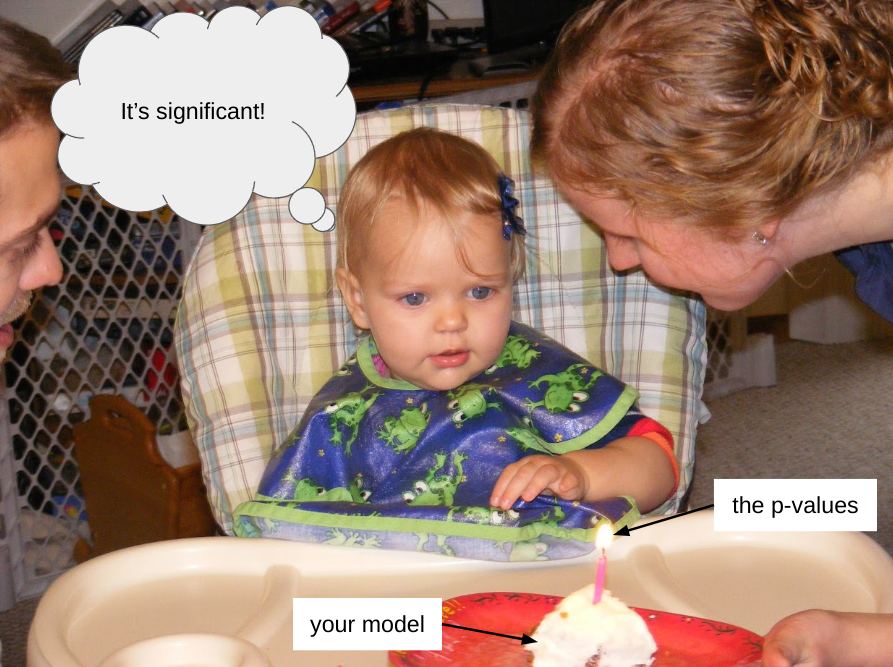
\includegraphics{./cake.png}
\caption{Baby Ellie examines her model.}
\end{figure}

\hypertarget{checkpoint}{%
\section{Checkpoint}\label{checkpoint}}

My guess is that what we have covered so far was perhaps mildly
uncomfortable but familiar. Some of you already have a lot of experience
fitting multiple regression models and visualizing them with
\texttt{ggeffects}. That's good. Now you can articulate that procedure
in terms of marginal and conditional effects.

You probably have questions, though. What about post-hoc tests?
Interactions? Models with nonlinearities? Random effects?

Stand by.

\hypertarget{when-model-parameters-are-not-enough}{%
\section{When model parameters are not
enough}\label{when-model-parameters-are-not-enough}}

As models become more complex, parameter estimates alone become hard or
impossible to interpret, and the notion of marginal and conditional
effects becomes more complicated (and eventually contradictory). Let's
consider two kinds of models that we use a lot in ecology: GAMs and
interaction models.

\hypertarget{gams}{%
\subsection{GAMs}\label{gams}}

None of the variables in the penguins data set have curvy relationships,
so we'll have to cheat a bit. If we take only the Chinstrap and Adelie
species and plot \texttt{body\ mass} against \texttt{bill\_length},
ignoring species, we get a curvy shape. Again, this is just to give us
something to fit a GAM to.

\begin{Shaded}
\begin{Highlighting}[]
\NormalTok{data }\OtherTok{\textless{}{-}}\NormalTok{ penguins }\SpecialCharTok{\%\textgreater{}\%}
  \FunctionTok{filter}\NormalTok{(species }\SpecialCharTok{\%in\%} \FunctionTok{c}\NormalTok{(}\StringTok{"Adelie"}\NormalTok{, }\StringTok{"Chinstrap"}\NormalTok{)) }\SpecialCharTok{\%\textgreater{}\%}
  \FunctionTok{select}\NormalTok{(bill\_length\_mm, body\_mass\_g)}

\FunctionTok{ggplot}\NormalTok{(data, }\FunctionTok{aes}\NormalTok{(body\_mass\_g, bill\_length\_mm)) }\SpecialCharTok{+}
  \FunctionTok{geom\_point}\NormalTok{() }\SpecialCharTok{+}
  \FunctionTok{geom\_smooth}\NormalTok{() }\SpecialCharTok{+}
  \FunctionTok{theme\_lucid}\NormalTok{()}
\end{Highlighting}
\end{Shaded}

\includegraphics{demo_files/figure-latex/unnamed-chunk-16-1.pdf}

We'll fit a very simple GAM in which \texttt{bill\ length} is smooth
function of \texttt{body\ mass}. Please don't take this as an example of
how to fit GAMs. The goal is just to demonstrate a problem.

\begin{Shaded}
\begin{Highlighting}[]
\NormalTok{mod}\FloatTok{.02} \OtherTok{\textless{}{-}} \FunctionTok{gam}\NormalTok{(bill\_length\_mm }\SpecialCharTok{\textasciitilde{}} \FunctionTok{s}\NormalTok{(body\_mass\_g),}
              \AttributeTok{data =}\NormalTok{ data)}
\end{Highlighting}
\end{Shaded}

We tidy the model up, and right away we see the problem. Where is the
\(\beta\) coefficient? How are we supposed to get a marginal effect out
of this model?

\begin{Shaded}
\begin{Highlighting}[]
\NormalTok{mod}\FloatTok{.02}\NormalTok{\_estimates }\OtherTok{\textless{}{-}} \FunctionTok{tidy}\NormalTok{(mod}\FloatTok{.02}\NormalTok{)}
\NormalTok{mod}\FloatTok{.02}\NormalTok{\_estimates}
\end{Highlighting}
\end{Shaded}

\begin{verbatim}
## # A tibble: 1 x 5
##   term             edf ref.df statistic   p.value
##   <chr>          <dbl>  <dbl>     <dbl>     <dbl>
## 1 s(body_mass_g)  1.91   2.41      10.4 0.0000192
\end{verbatim}

If we visualize the model, the nature of the problem becomes obvious.
The slope of \texttt{bill\ length\ \textasciitilde{}\ body\ mass} is not
a constant; it changes depending on where you are along the x-axis of
\texttt{body\ mass}. What could the marginal effect of
\texttt{body\ mass} even \emph{mean} in a model like this?

\begin{Shaded}
\begin{Highlighting}[]
\NormalTok{mod}\FloatTok{.02}\NormalTok{\_predictions }\OtherTok{\textless{}{-}} \FunctionTok{ggpredict}\NormalTok{(mod}\FloatTok{.02}\NormalTok{)}
\FunctionTok{plot}\NormalTok{(mod}\FloatTok{.02}\NormalTok{\_predictions)}
\end{Highlighting}
\end{Shaded}

\begin{verbatim}
## $body_mass_g
\end{verbatim}

\includegraphics{demo_files/figure-latex/unnamed-chunk-19-1.pdf}

Hold that thought while we consider another problem.

\hypertarget{interactions}{%
\subsection{Interactions}\label{interactions}}

Now consider a slightly more serious model. Let's say we're
reconsidering \texttt{mod\_01}, and we really think it should include an
\emph{interaction} between our factor \texttt{species} and our
continuous variables \texttt{flipper\ length}. For simplicity, we'll
drop \texttt{body\ mass} from this model.

\begin{Shaded}
\begin{Highlighting}[]
\NormalTok{mod}\FloatTok{.03} \OtherTok{\textless{}{-}} \FunctionTok{lm}\NormalTok{(bill\_depth\_mm }\SpecialCharTok{\textasciitilde{}}
\NormalTok{               flipper\_length\_mm }\SpecialCharTok{+}
\NormalTok{               species }\SpecialCharTok{+}
\NormalTok{               flipper\_length\_mm}\SpecialCharTok{:}\NormalTok{species,}
             \AttributeTok{data =}\NormalTok{ penguins)}
\end{Highlighting}
\end{Shaded}

Tidy it up and inspect the parameter estimates. We have a \(\beta\)
coefficient for \texttt{flipper\ length}, \(\beta\) coefficients for the
\texttt{species} levels of Chinstrap and Gentoo, and then \(\beta\)
coefficients for \texttt{flipper\ length\ :\ Chinstrap} and
\texttt{flipper\ length\ :\ Gentoo}. Can we understand these \(\beta\)
coefficients as marginal/conditional effects?

\begin{Shaded}
\begin{Highlighting}[]
\NormalTok{mod}\FloatTok{.03}\NormalTok{\_estimates }\OtherTok{\textless{}{-}} \FunctionTok{tidy}\NormalTok{(mod}\FloatTok{.03}\NormalTok{)}
\NormalTok{mod}\FloatTok{.03}\NormalTok{\_estimates}
\end{Highlighting}
\end{Shaded}

\begin{verbatim}
## # A tibble: 6 x 5
##   term                               estimate std.error statistic    p.value
##   <chr>                                 <dbl>     <dbl>     <dbl>      <dbl>
## 1 (Intercept)                          7.47      2.31        3.24 0.00131   
## 2 flipper_length_mm                    0.0572    0.0121      4.72 0.00000350
## 3 speciesChinstrap                    -7.14      3.99       -1.79 0.0747    
## 4 speciesGentoo                      -15.7       3.74       -4.20 0.0000344 
## 5 flipper_length_mm:speciesChinstrap   0.0351    0.0206      1.71 0.0890    
## 6 flipper_length_mm:speciesGentoo      0.0497    0.0182      2.73 0.00667
\end{verbatim}

Let's look at them one at a time.

\begin{center}\rule{0.5\linewidth}{0.5pt}\end{center}

\(\beta_0\): Just like in \texttt{mod.01}, the intercept represents
\texttt{bill\_depth} when \texttt{species\ =\ Adelie} and
\texttt{flipper\ length\ =\ 0}.

\(\beta_1\): This is the slope of
\texttt{bill\ depth\ \textasciitilde{}\ flipper\ length}, but there's a
catch. In \texttt{mod.01}, which did not have interactions, this slope
was assumed to be the same across all values of the covariates. In this
interaction model, that is no longer true; this parameter is the slope
of \texttt{bill\ depth\ \textasciitilde{}\ flipper\ length} \emph{only}
for \texttt{species\ =\ Adelie}. We can no longer consider this a
marginal effect the way we did in \texttt{mod.01}.

\(\beta_2\): As in \texttt{mod01}, this is the change in
\texttt{bill\ depth} when you go from \texttt{species\ =\ Adelie} to
\texttt{species\ =\ Chinstrap}, conditional on \texttt{flipper\ length}
being set to its mean. This difference is the \textbf{conditional
effect} of \texttt{species\ =\ Chinstrap} on \texttt{bill\ depth}.

\(\beta_3\): Same as above, but for Gentoo.

Now things get tricky.

\(\beta_4\): This is the value that gets \emph{added} to \(\beta_1\) to
give you the slope of
\texttt{bill\ depth\ \textasciitilde{}\ flipper\ length} given
\texttt{species\ =\ Chinstrap}.

\(\beta_5\): This is the value that gets \emph{added} to \(\beta_1\) to
give you the slope of
\texttt{bill\ depth\ \textasciitilde{}\ flipper\ length} given
\texttt{species\ =\ Gentoo}.

\begin{center}\rule{0.5\linewidth}{0.5pt}\end{center}

This is problematic. We have \textbf{conditional} effects for species,
but none of the \(\beta\) coefficients can be interpreted as a
\textbf{marginal} effect of \texttt{flipper\ length}. What do we do?

\hypertarget{mixed-effects}{%
\subsection{Mixed effects}\label{mixed-effects}}

Now let's consider one more kind of model that complicates our notion of
marginal effects: a mixed-effect model. Returning to our penguin data,
let's use \texttt{species} as a random intercept rather than a fixed
effect. Again, for simplicity \texttt{flipper\ length} will be the only
continuous variable we consider.

The math of a mixed effects model looks like this:

\[ bill.depth \sim \mathcal{N}(\mu_j, \sigma_y) \]

The subscript in \(\mu_j\) tells us that \(\mu\) varies with \(j\),
which in our model is \texttt{species}. Specifically, the intercept
\(\beta_0\) gets a value \(b_{0_j}\) added to it for each level of
species.

\[ \mu =  (\beta_0 + b_{0_j}) + \beta_1flipper.length \]

The value added to the intercept to represent species-level variation is
drawn from a normal distribution with mean = 0 and a standard deviation
estimated from the data:

\[b_{0_j} \sim \mathcal{N}(0, \sigma_0)\]

Honestly, I'm shaky on the math here, but it's close enough for our
purposes. Let's fit the model.

\begin{Shaded}
\begin{Highlighting}[]
\NormalTok{mod}\FloatTok{.04} \OtherTok{\textless{}{-}} \FunctionTok{lmer}\NormalTok{(bill\_depth\_mm }\SpecialCharTok{\textasciitilde{}}\NormalTok{ flipper\_length\_mm }\SpecialCharTok{+}\NormalTok{ (}\DecValTok{1} \SpecialCharTok{|}\NormalTok{ species),}
               \AttributeTok{data =}\NormalTok{ penguins)}
\end{Highlighting}
\end{Shaded}

Unfortunately, we cannot use \texttt{tidy()} on a mixed effects model,
but we can use the lovely \texttt{modelsummary()} function from
\texttt{marginaleffects} to get a neat overview of our parameter
estimates.

\begin{Shaded}
\begin{Highlighting}[]
\FunctionTok{modelsummary}\NormalTok{(mod}\FloatTok{.04}\NormalTok{)}
\end{Highlighting}
\end{Shaded}

\begin{table}
\centering
\begin{tabular}[t]{lc}
\toprule
  & (1)\\
\midrule
(Intercept) & \num{0.829}\\
 & (\num{2.415})\\
flipper\_length\_mm & \num{0.082}\\
 & (\num{0.008})\\
SD (Intercept species) & \num{3.117}\\
SD (Observations) & \num{0.980}\\
\midrule
Num.Obs. & \num{342}\\
R2 Marg. & \num{0.110}\\
R2 Cond. & \num{0.920}\\
AIC & \num{988.6}\\
BIC & \num{1003.9}\\
ICC & \num{0.9}\\
RMSE & \num{0.97}\\
\bottomrule
\end{tabular}
\end{table}

What can we make of this? Well, the \textbf{marginal effect} of
\texttt{flipper\ length} is simple enough --- it's just \(\beta_1\), the
same as in \texttt{mod.01}. But what if we want \textbf{marginal means}?
How do we account for the variation in the random effects term
\(b_{0_j}\)? Or should we just ignore it?

\texttt{ggeffects} gives us a couple of options. The default behavior is
to ignore the random effect and plot the predictions based only on the
fixed terms. But we can also choose to incorporate the uncertainty
arising from the random effect. Let's see how this affects our results.

\begin{Shaded}
\begin{Highlighting}[]
\CommentTok{\# Fixed only}
\NormalTok{mod}\FloatTok{.04}\NormalTok{\_predictions\_fixed }\OtherTok{\textless{}{-}} \FunctionTok{ggpredict}\NormalTok{(mod}\FloatTok{.04}\NormalTok{)}\SpecialCharTok{$}\NormalTok{flipper\_length\_mm }\SpecialCharTok{\%\textgreater{}\%}
  \FunctionTok{tibble}\NormalTok{() }\SpecialCharTok{\%\textgreater{}\%}
  \FunctionTok{mutate}\NormalTok{(}\AttributeTok{model =} \StringTok{"fixed"}\NormalTok{)}

\CommentTok{\# With random}
\NormalTok{mod}\FloatTok{.04}\NormalTok{\_predictions\_random }\OtherTok{\textless{}{-}} \FunctionTok{ggpredict}\NormalTok{(mod}\FloatTok{.04}\NormalTok{, }\AttributeTok{type =} \StringTok{"re"}\NormalTok{)}\SpecialCharTok{$}\NormalTok{flipper\_length\_mm }\SpecialCharTok{\%\textgreater{}\%}
  \FunctionTok{tibble}\NormalTok{() }\SpecialCharTok{\%\textgreater{}\%}
  \FunctionTok{mutate}\NormalTok{(}\AttributeTok{model =} \StringTok{"random"}\NormalTok{)}

\CommentTok{\# Collate}
\NormalTok{mod}\FloatTok{.04}\NormalTok{\_predictions }\OtherTok{\textless{}{-}} \FunctionTok{bind\_rows}\NormalTok{(mod}\FloatTok{.04}\NormalTok{\_predictions\_fixed, }
\NormalTok{                                mod}\FloatTok{.04}\NormalTok{\_predictions\_random) }\SpecialCharTok{\%\textgreater{}\%}
  \FunctionTok{mutate}\NormalTok{(}\AttributeTok{model =} \FunctionTok{factor}\NormalTok{(model, }\AttributeTok{levels =} \FunctionTok{c}\NormalTok{(}\StringTok{"random"}\NormalTok{, }\StringTok{"fixed"}\NormalTok{)))}
\end{Highlighting}
\end{Shaded}

First, notice that the fit lines for the two types of prediction are
identical. This is because the line is based solely on \(\beta_1\) in
both cases. What differs is the uncertainty around this estimate. When
we ignore the random effect, we get a tighter confidence interval. In
this case, because the random effect happens to be weak, the difference
is very small, but it can be much more pronounced in models with
stronger random effects.

\begin{Shaded}
\begin{Highlighting}[]
\FunctionTok{ggplot}\NormalTok{(mod}\FloatTok{.04}\NormalTok{\_predictions, }\FunctionTok{aes}\NormalTok{(x, predicted, }
                               \AttributeTok{ymin =}\NormalTok{ conf.low, }
                               \AttributeTok{ymax =}\NormalTok{ conf.high,}
                               \AttributeTok{fill =}\NormalTok{ model)) }\SpecialCharTok{+}
  \FunctionTok{geom\_ribbon}\NormalTok{(}\AttributeTok{alpha =} \FloatTok{0.5}\NormalTok{) }\SpecialCharTok{+}
  \FunctionTok{geom\_line}\NormalTok{() }\SpecialCharTok{+}
  \FunctionTok{labs}\NormalTok{(}\AttributeTok{x =} \StringTok{"flipper\_length\_mm"}\NormalTok{, }\AttributeTok{y =} \StringTok{"bill\_depth\_mm"}\NormalTok{) }\SpecialCharTok{+}
  \FunctionTok{theme\_lucid}\NormalTok{()}
\end{Highlighting}
\end{Shaded}

\includegraphics{demo_files/figure-latex/unnamed-chunk-25-1.pdf}

Which is the right choice? And which one can be called a ``marginal
mean''?

\hypertarget{the-horrible-mess-defining-marginal-and-conditional-effects}{%
\section{The horrible mess: defining marginal and conditional
effects}\label{the-horrible-mess-defining-marginal-and-conditional-effects}}

We need to revisit the definitions of marginal and conditional effects
in light of the models presented above. If it's not still fresh in your
mind, reread that email correspondence that I had with Andrew Heiss. The
unfortunate truth is that there are \textbf{at least three mutually
incompatible definitions} of marginal and conditional effects floating
around the world of statisticians and practitioners. We can't fix the
terminology, but we can understand the different meanings that the terms
can have, and how they relate to different types of models.

\textbf{1. Sliders vs.~switches}

This is the definition I introduced with \texttt{mod.01}: a marginal
effect is the (partial) slope on the response variable on a continuous
predictor
(e.g.~\texttt{bill\_depth\ \textasciitilde{}\ flipper\ length}), and a
conditional effect is the change in the response variable when a
categorical variable goes from its reference level
(e.g.~\texttt{species\ =\ Adelie}) to some other level
(e.g.~\texttt{species\ =\ Gentoo}). This, I think, happens to be the
classical definition that real statisticians usually have in mind. For
an excellent overview of this sense of marginal and conditional effects,
see Andrew Heiss'
\href{https://www.andrewheiss.com/blog/2022/05/20/marginalia/}{``Marginalia''}.

\textbf{2. Conditioning vs.~averaging}

This definition comes into play when your model has interactions (or
random slopes). Under this definition, a marginal effect averages
\(\beta\) parameters over an interacting covariate, while a conditional
effect fixes the interacting covariate at a specified level. For
example, in \texttt{mod.03}, the marginal effect of
\texttt{flipper\ length} would be the average (or potentially some other
summary) of the species-specific slopes, thus representing the slope
expected for a hypothetical species that is the average of the three
observed species. The conditional effect of \texttt{flipper\ length}
would be the slope given a specific level of species, say
\texttt{species\ =\ Chinstrap}. Thus, in that model, there would be only
one marginal effect of \texttt{flipper\ length} but three conditional
effects, one for each level of \texttt{species}.

\textbf{3. Incorporating vs.~ignoring random effects}

Finally, in the context of mixed effect models, the terms ``marginal''
and ``conditional'' take on yet a third meaning with respect to
\emph{predictions}. Marginal means are based on predictions that
incorporate the uncertainty arising from the random effects component of
the model, while conditional means are based on predictions that use
only the fixed terms of the model. Thus, conditional means will
generally have tighter confidence intervals that marginal means. When it
comes to interpretation, a marginal mean can be understood as the
expected value for a randomly selected penguin that belongs to one of
the 3 species, but you don't know which one. This uncertainty is
reflected in the wider confidence interval, which has to cover the full
range of possibility comprised by Adelie, Chinstrap, and Gentoo
penguins. In contrast, a conditional mean can be understood as the
expected value for a hypothetical average penguin, an Adelchintoo, if
you will.

Each of these definitions is, by itself, useful and legitimate. The
problem, of course, is that they cannot be reconciled with each other.
Whenever you use the term ``marginal'' or ``conditional,'' it is up to
you to understand which of these definitions you are working with, to
align this usage with the interpretation of your models, and to
communicate all this clearly to your audience.

\begin{figure}
\centering
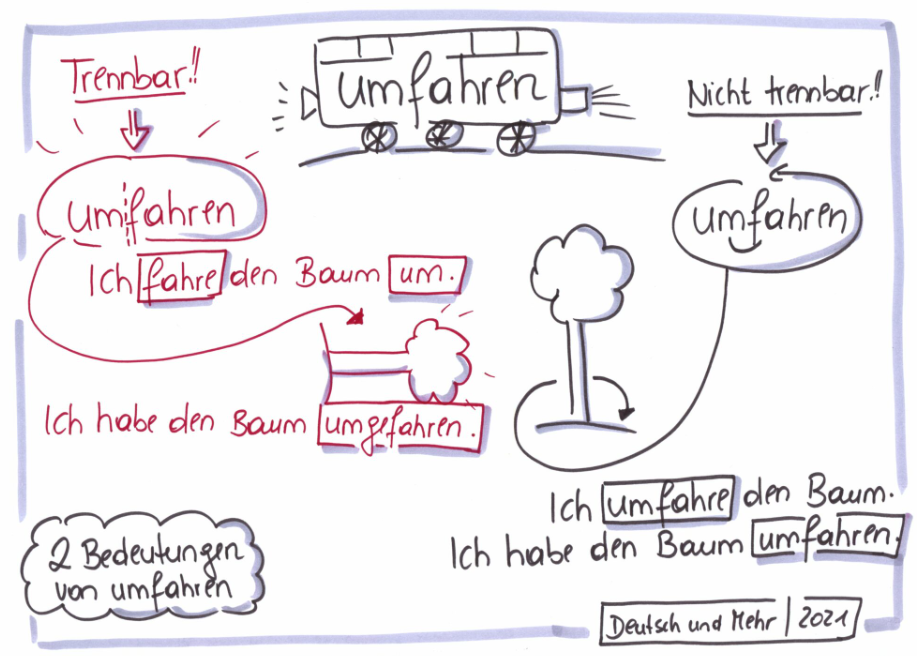
\includegraphics{./umfahren.png}
\caption{\url{https://sketchnotes.at/sketchnotes/umfahren-oder-doch-umfahren/}}
\end{figure}

\hypertarget{introducing-marginaleffects}{%
\section{\texorpdfstring{Introducing
\texttt{marginaleffects}}{Introducing marginaleffects}}\label{introducing-marginaleffects}}

\end{document}
